\subsection{\label{sec:calib.tof}Time-of-Flight Counter Calibration and Resolution}

\subsubsection{\label{sec:calib.tof.eff}Time-of-Flight Counter Efficiency and Bad Paddles}

As a standard procedure of the time-of-flight calibrations, the time-of-flight scintillators were initially studied during the calibration period, in which a list~\footnote{Can be obtained using the CLAS calibration database} of scintillators had a faulty ADC or TDC as shown in \ref{tab:craigtof}. Another study, as shown below, was conducted to determine the efficiency of each paddle and to reevaluate the status of their ADC and TDC. Due to the more stringent requirements of paddle efficiency in the study below, more paddles were considered to be faulty than in the initial study. \ref{tab:diff} shows the additional paddles which were considered to be inefficient.

\begin{table}
\begin{minipage}{\textwidth}
\begin{center}
\begin{singlespacing}

\caption{\label{tab:craigtof}List of faulty paddles as compiled during calibration}
    
\begin{tabular}{llp{.43\textwidth}}

\hline \hline

Sector & SCID & Notes \\

\hline

1 & 6 & No ADCR and TDCR \\
2 & 8 & No ADCL and TDCL \\
2 & 34 & No ADCL and TDCL \\
3 & 11 & No ADCR and TDCR \\
3 & 57 & No ADCL, ADCR, TDCL, and TDCR \\
4 & 48 & No ADCL and TDCL \\
5 & 57 & No ADCL, ADCR, TDCL, and TDCR \\
6 & 5 & No ADCR and TDCR \\

\hline \hline

\end{tabular}

\end{singlespacing}
\end{center}
\end{minipage}
\end{table}
 % label: tab:craigtof

\begin{figure}
    %\vspace{16pt}
    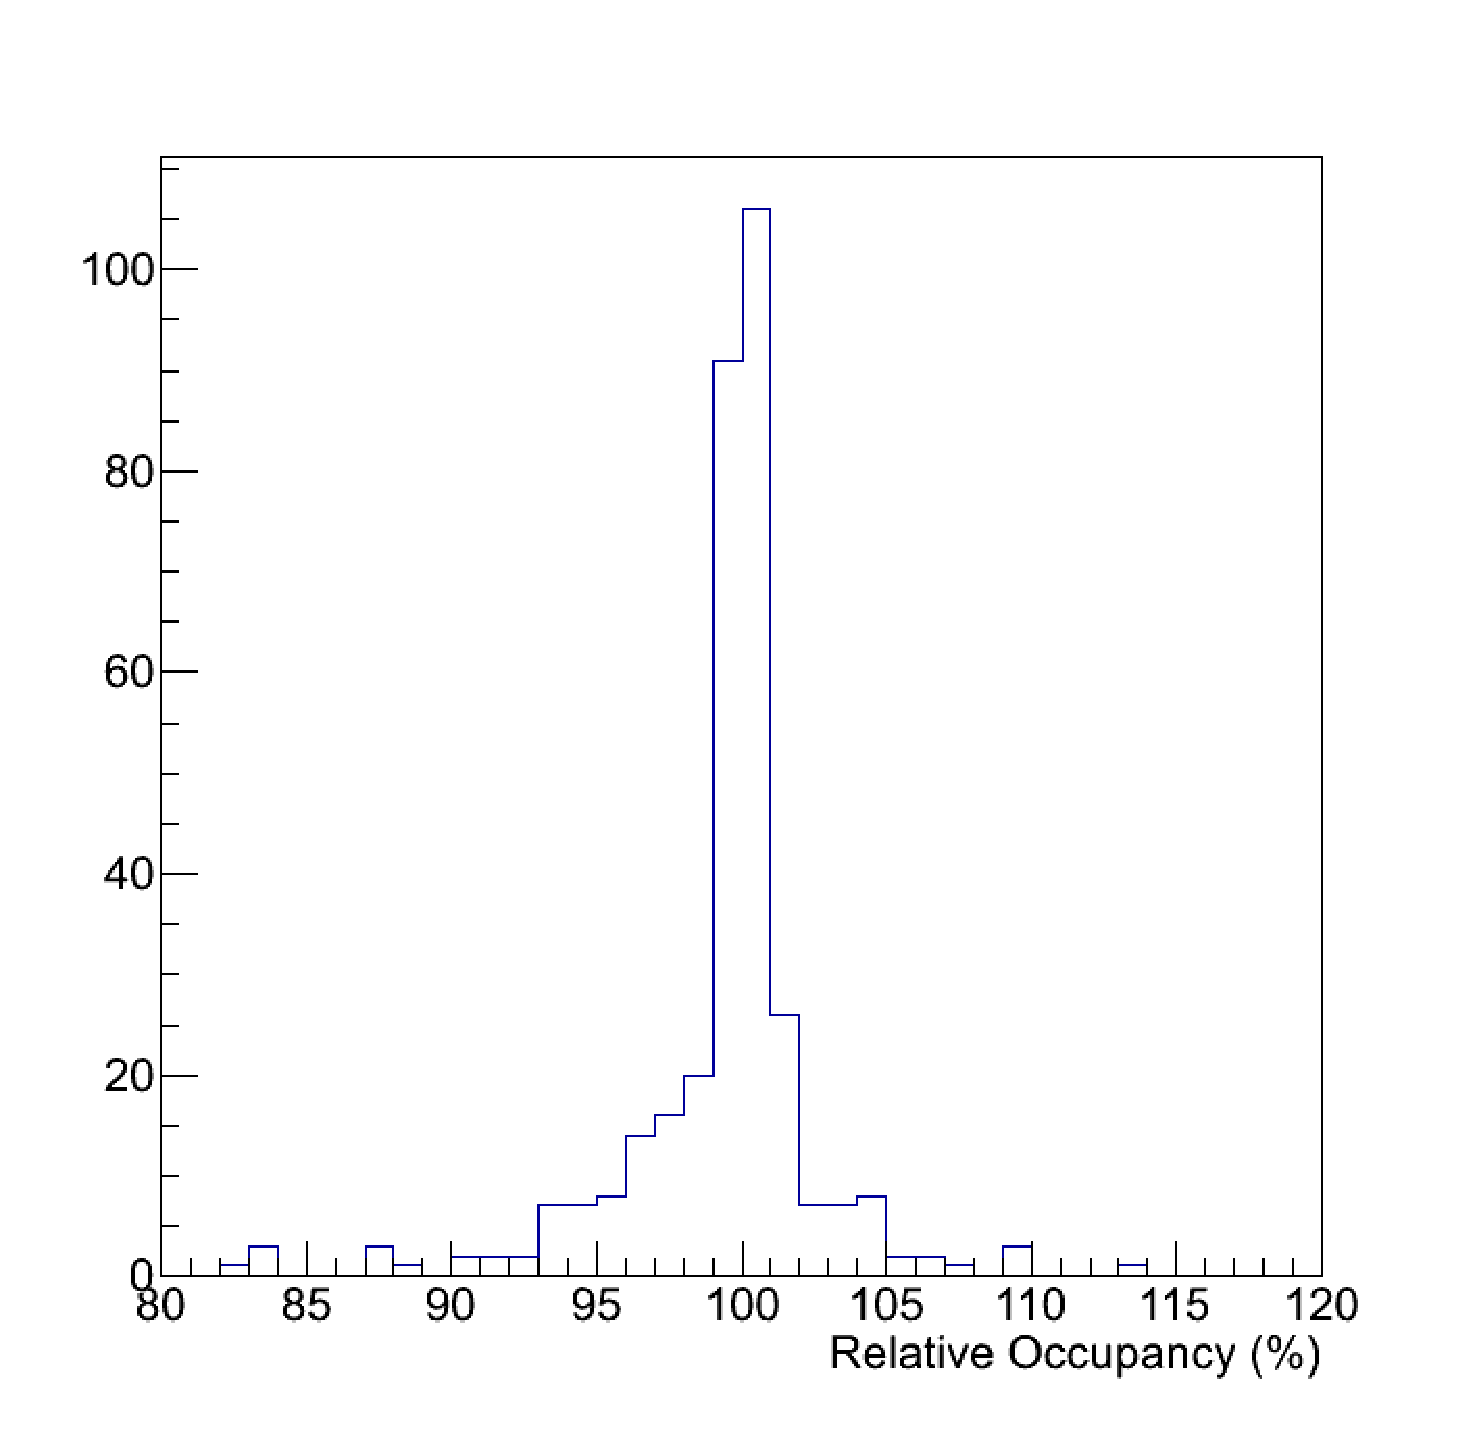
\includegraphics[trim=0 40 10 40,clip,width=.70\linewidth]{figures/calib/tof/tofko/occp.eps}
    \caption{Relative occupancy of all scintillators}
    \label{plt:occp}
\end{figure}

To determine efficiency of each scintillator paddle, the number of hits~\footnote{The data used were obtained from the \texttt{clas\underline{\hspace{5pt}}0$[$run\#$]$.A01} files located in \texttt{$/$mss$/$clas$/$g12$/$data$/$}} registered by every paddle was recorded~\footnote{This was done by using \texttt{bosdump -GSC} and parsing its output}. The relative occupancy of paddle $i$ in sector $j$ is defined the following way: list the number of hits recorded by all paddle $i$'s in sectors $\neq j$ and remove the ones with the most and least hits from the list. Take the average number of hits of the remaining three paddles. The relative occupancy is defined as 
\[
100 \times \frac{ \mathrm{Number of hits in paddle } i \mathrm{ of sector } j}{\mathrm{Average of remaining three paddles}} \hspace{2pt}\%
\]

\ref{plt:occp} shows the relative occupancy of all scintillators plotted on a single histogram. A paddle is defined as inefficient if it is greater than two standard deviations below the mean relative occupancy of all scintillators. \ref{tab:occp} shows the paddles which are below two (left) or three (right) standard deviations below the mean relative occupancy.


\input{tables/tof_padpaddles_stddev} % label: tab:occp

\subsubsection{ADC and TDC Values}


\begin{figure}
    %\vspace{-16pt}
    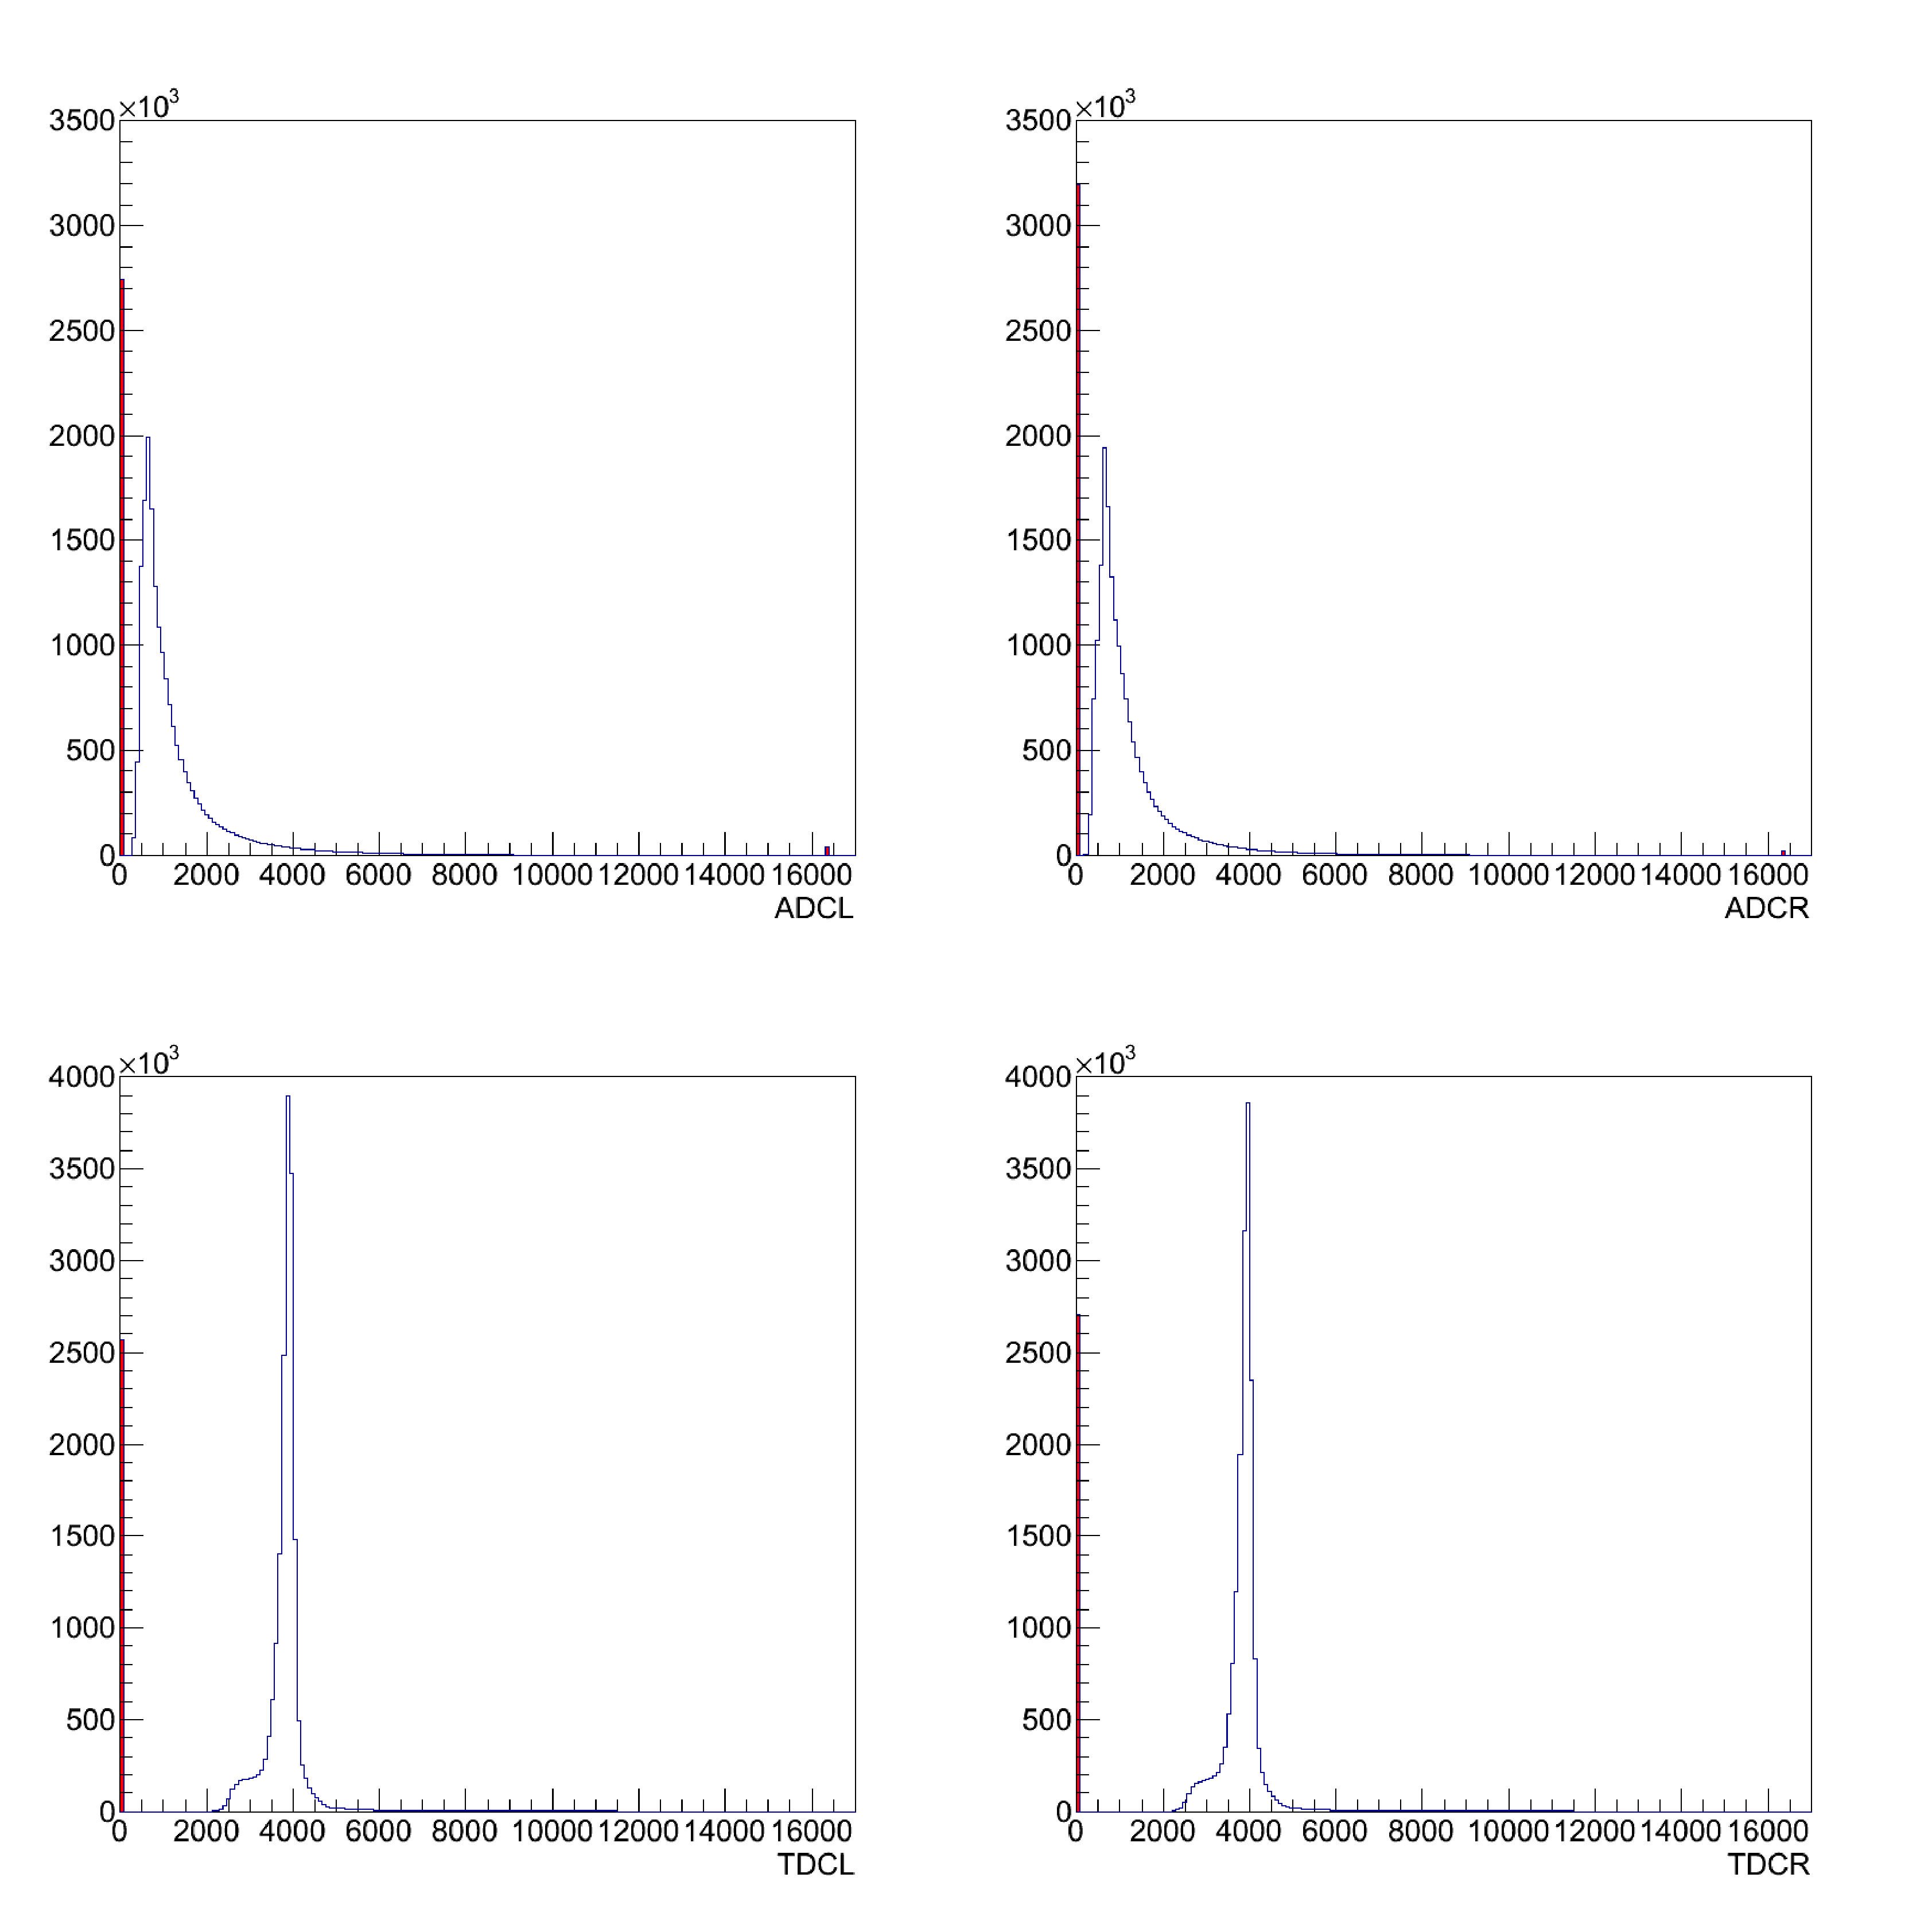
\includegraphics[width=0.70\linewidth]{figures/calib/tof/tofko/adctdcval.eps}
    \caption{Top: ADC values of all scintillators. Left ADC (ADCL) values are on the left and right ADC values are on the right (ADCR). Shaded in red are events recorded with an ADC value of zero or maximum. Bottom: Same as Top but for TDC values}
    \label{plt:adctdcval}
\end{figure}


The occupancy alone is not enough to determine which scintillators are bad. The ADC and TDC values for all scintillators were also recorded and studied. \ref{plt:adctdcval} shows the ADC and TDC values for all scintillators. Some of the events registered had an ADC or TDC value of zero or a maximum ADC value (shaded in red). The percentage of events a scintillator recorded either a TDC or ADC value of zero or maximum ADC value was studied as shown in \ref{plt:adc0vSCID,plt:adcMvSCID,plt:tdc0vSCID}. \ref{plt:adc0vSCID,plt:tdc0vSCID,plt:proj} assisted in determining bad paddles. It (is to be) was decided that a paddle cannot have more than $50\%$ of its ADC (left or right) values be equal to zero or more than $45\%$ of its TDC (left or right) values equal to zero. \ref{tab:adctdc0} shows which paddles fall in these categories. \ref{tab:tofko} shows which scintillators should be knocked out due to low occupancy or too many null ADC or TDC values. Due to the small number of events in which a maximum ADC value is obtained, it is not recommended in knocking paddles out based on this measure. However, \ref{tab:adcM} shows the paddles which attain a maximum ADC value on more than $2.5\%$ of its registered events.

\begin{table}
\begin{tabular}{l|p{.43\textwidth}|p{.43\textwidth}} %l | >{\centering\arraybackslash}p{.43\textwidth} | >{\centering\arraybackslash}p{.43\textwidth} |}
 &  \% Events with ADCL or ADCR = 0 \( > \) 50\% &  \% Event with TDCL or TDCR = 0 \( > \) 45\% \\ 
\hline
Sector 1 & 6 (100\% ADCR) & 6 (100\% TDCR), 46 (97.89\% TDCL), 50 (98.11\% TDCL) \\
Sector 2 & 8 (100\% ADCL), 34 (100\% ADCL), 44 (50.22\% ADCL), 54 (52.00\% ADCR) &  8 (100\% TDCL), 34 (100\% TDCL), 44 (47.51\% TDCL), 54 (47.10\% TDCR)\\
Sector 3 & 11 (100\% ADCR), 56 (74.75\% ADCR) & 11 (100\% TDCR), 56 (62.79\% TDCR)\\
Sector 4 & 48 (100\% ADCL) & 48 (100\% TDCL) \\
Sector 5 & 48 (77.98\% ADCL) & 48 (76.10\% TDCL)\\
Sector 6 & 5 (100\% ADCR), 56 (59.30\% ADCR) & 1 (98.78\% TDCL), 5 (100\% TDCR), 33 (97.78\% TDCL)
\end{tabular}
\caption{Paddles which registered an ADC or TDC value of zero greater than 50\% and 45\%, respectively, of its entries}
\label{tab:adctdc0}
\end{table}


\begin{table}
\centering
\begin{tabular}{l | c |}
Sector 1 & 6, 35, 40, 41, 50, 56\\
Sector 2 & 2, 8, 34, 35, 41, 44, 50, 54, 56\\
Sector 3 & 11, 35, 40, 41, 56\\
Sector 4 & 41, 48 \\
Sector 5 & 48\\
Sector 6 & 1, 5, 33, 56
\end{tabular}
\caption{Union of \ref{tab:occp,tab:adctdc0} (Recommended list of paddles to knockout)}
\label{tab:tofko}
\end{table}

\begin{table}
\centering
\begin{tabular}{l | c |}
Sector 1 & 35, 40, 41, 50, 56 \\
Sector 2 & 2, 35, 41, 44, 50, 54, 56 \\
Sector 3 & 35, 40, 41, 56 \\
Sector 4 & 41 \\
Sector 5 & 48 \\
Sector 6 & 1, 33, 56
\end{tabular}
\caption{Paddles in \ref{tab:tofko} not included in \ref{tab:craigtof}}
\label{tab:diff}
\end{table}

\begin{table}
\centering
\begin{tabular}{l | c |}
Sector 1 & 20 (2.93\% ADCL)\\
Sector 3 & 20 (4.26\% ADCL)
\end{tabular}
\caption{Paddles with percentage of hits registering a maximum ADC value \( > \) 2.5\% of its events}
\label{tab:adcM}
\end{table}

\begin{figure}
    %\vspace{-16pt}
    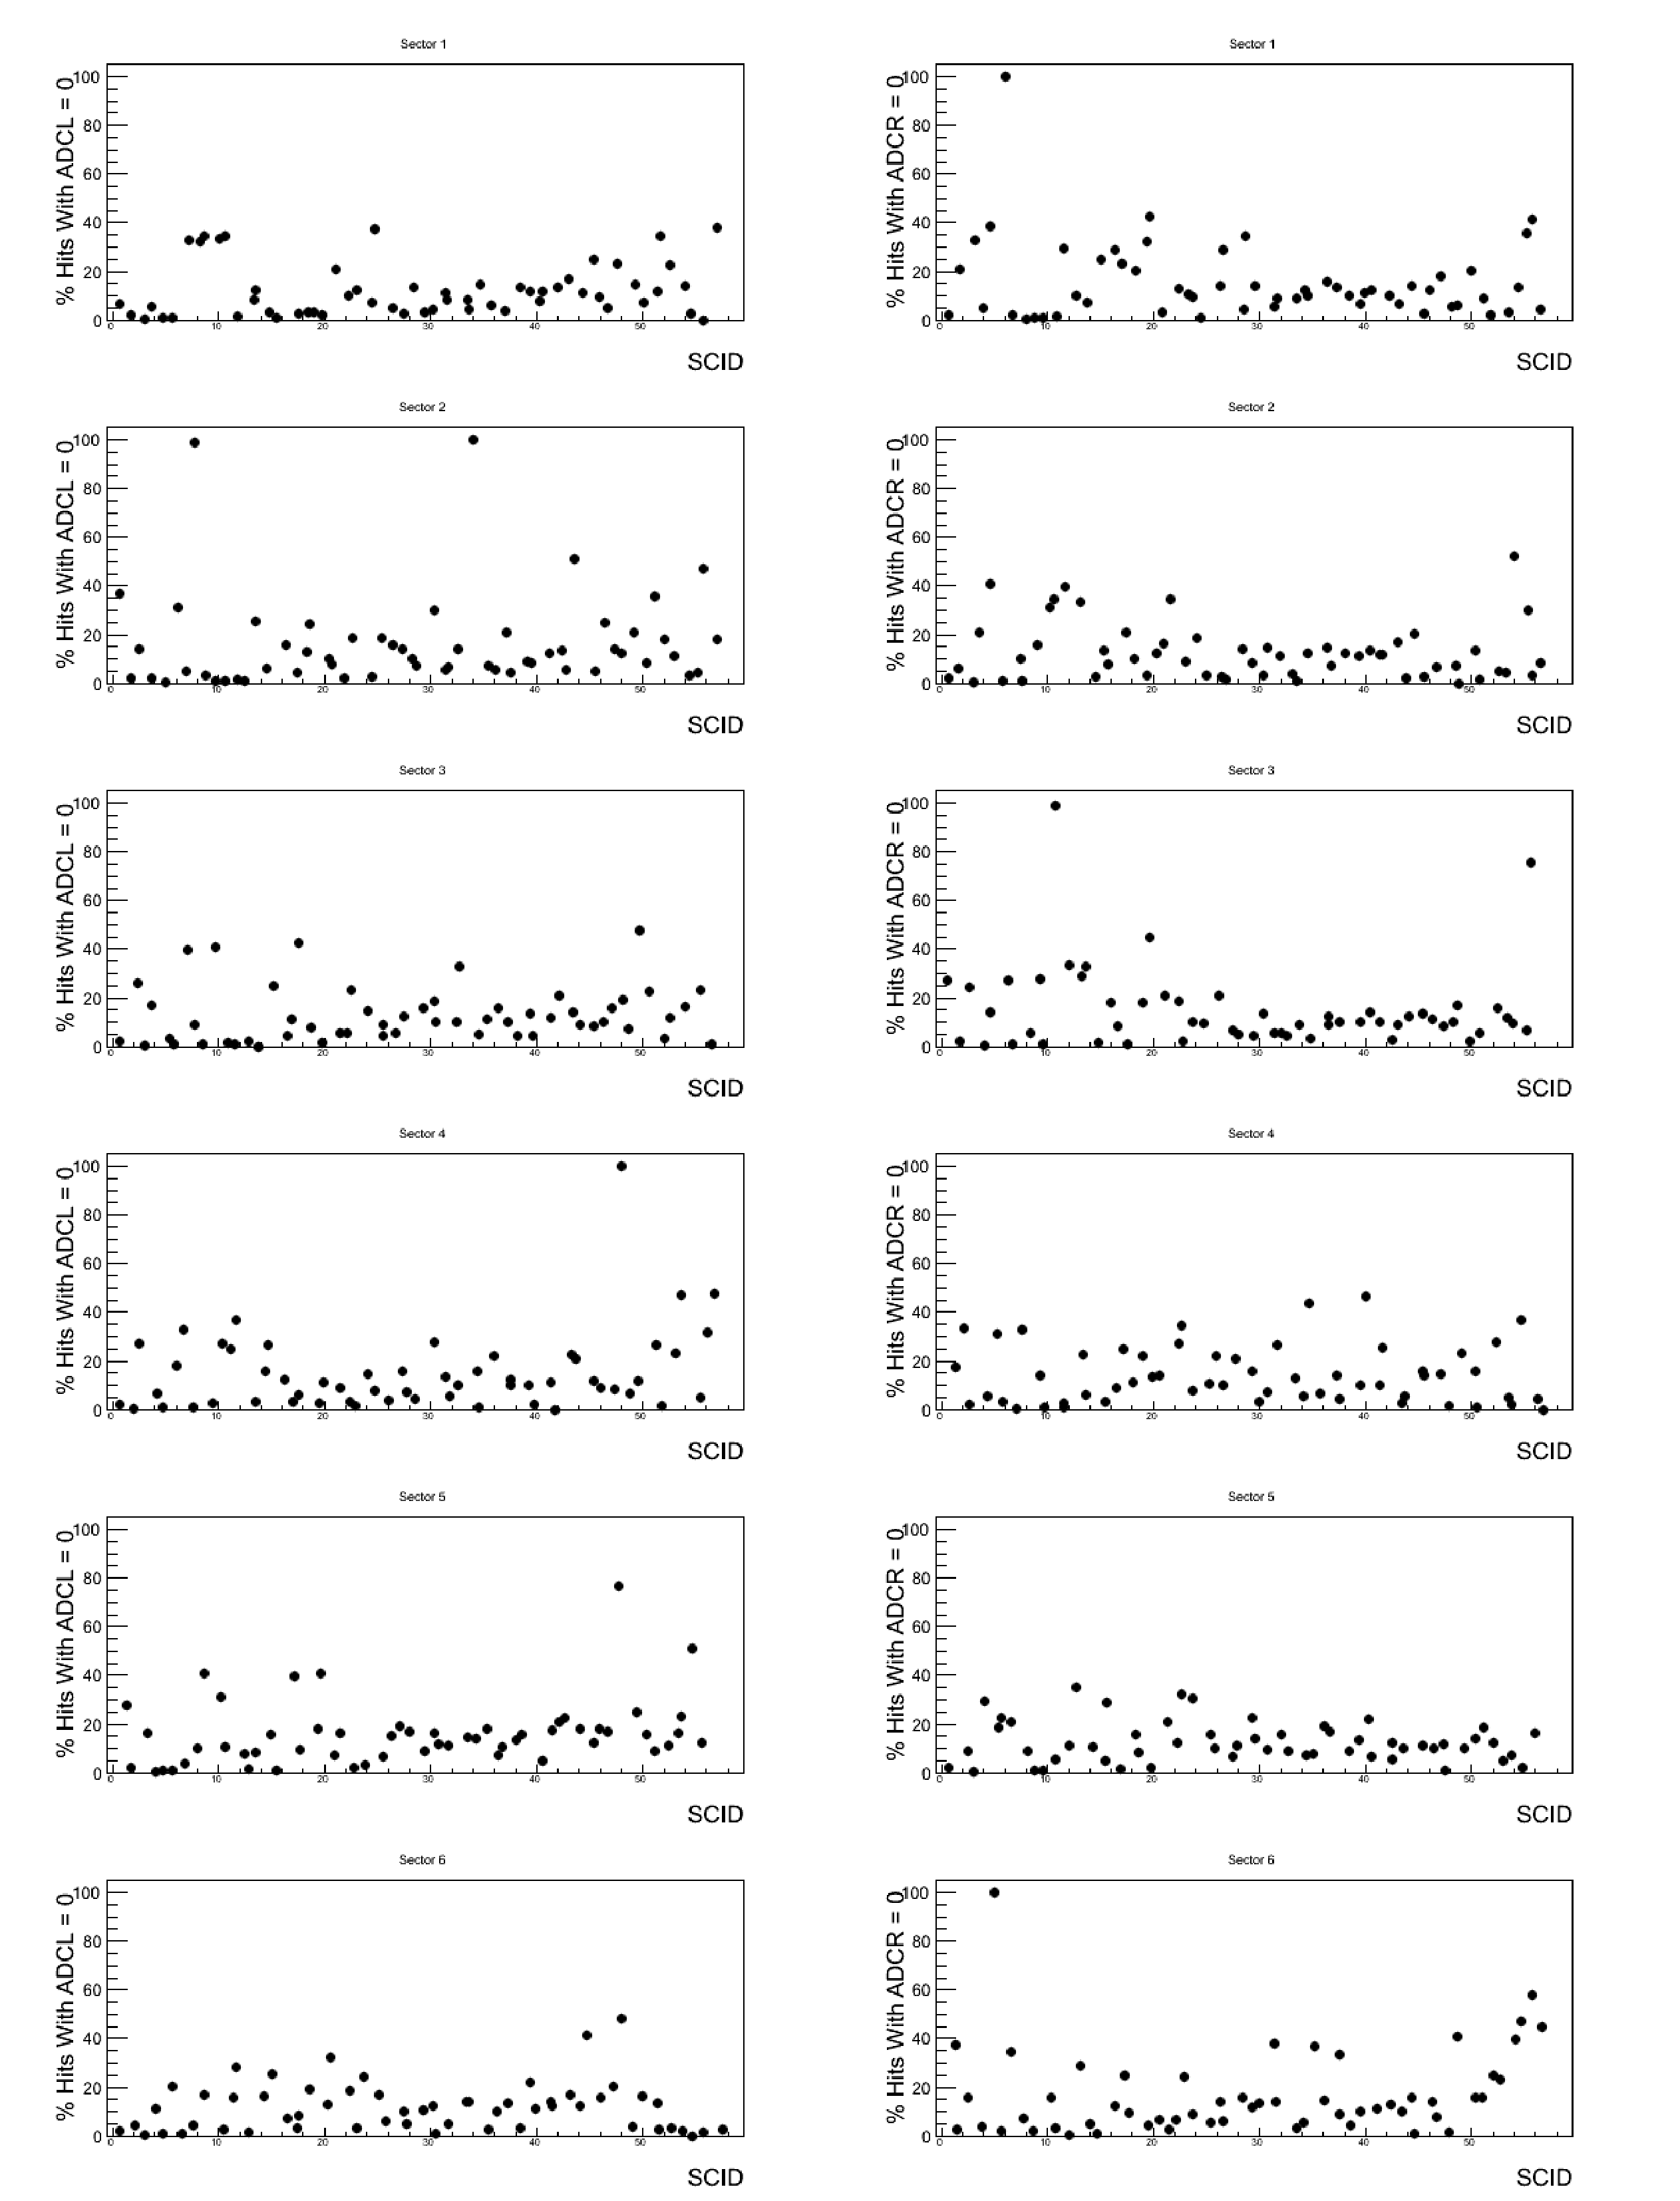
\includegraphics[width=0.8\textwidth]{figures/calib/tof/tofko/adc.eps}
    \caption{Percentage of hits registering an ADC value of 0 for all scintillators. Left ADC (ADCL) are on the left and right ADC (ADCR) values are on the right}
    \label{plt:adc0vSCID}
\end{figure}

\begin{figure}
    %\vspace{-16pt}
    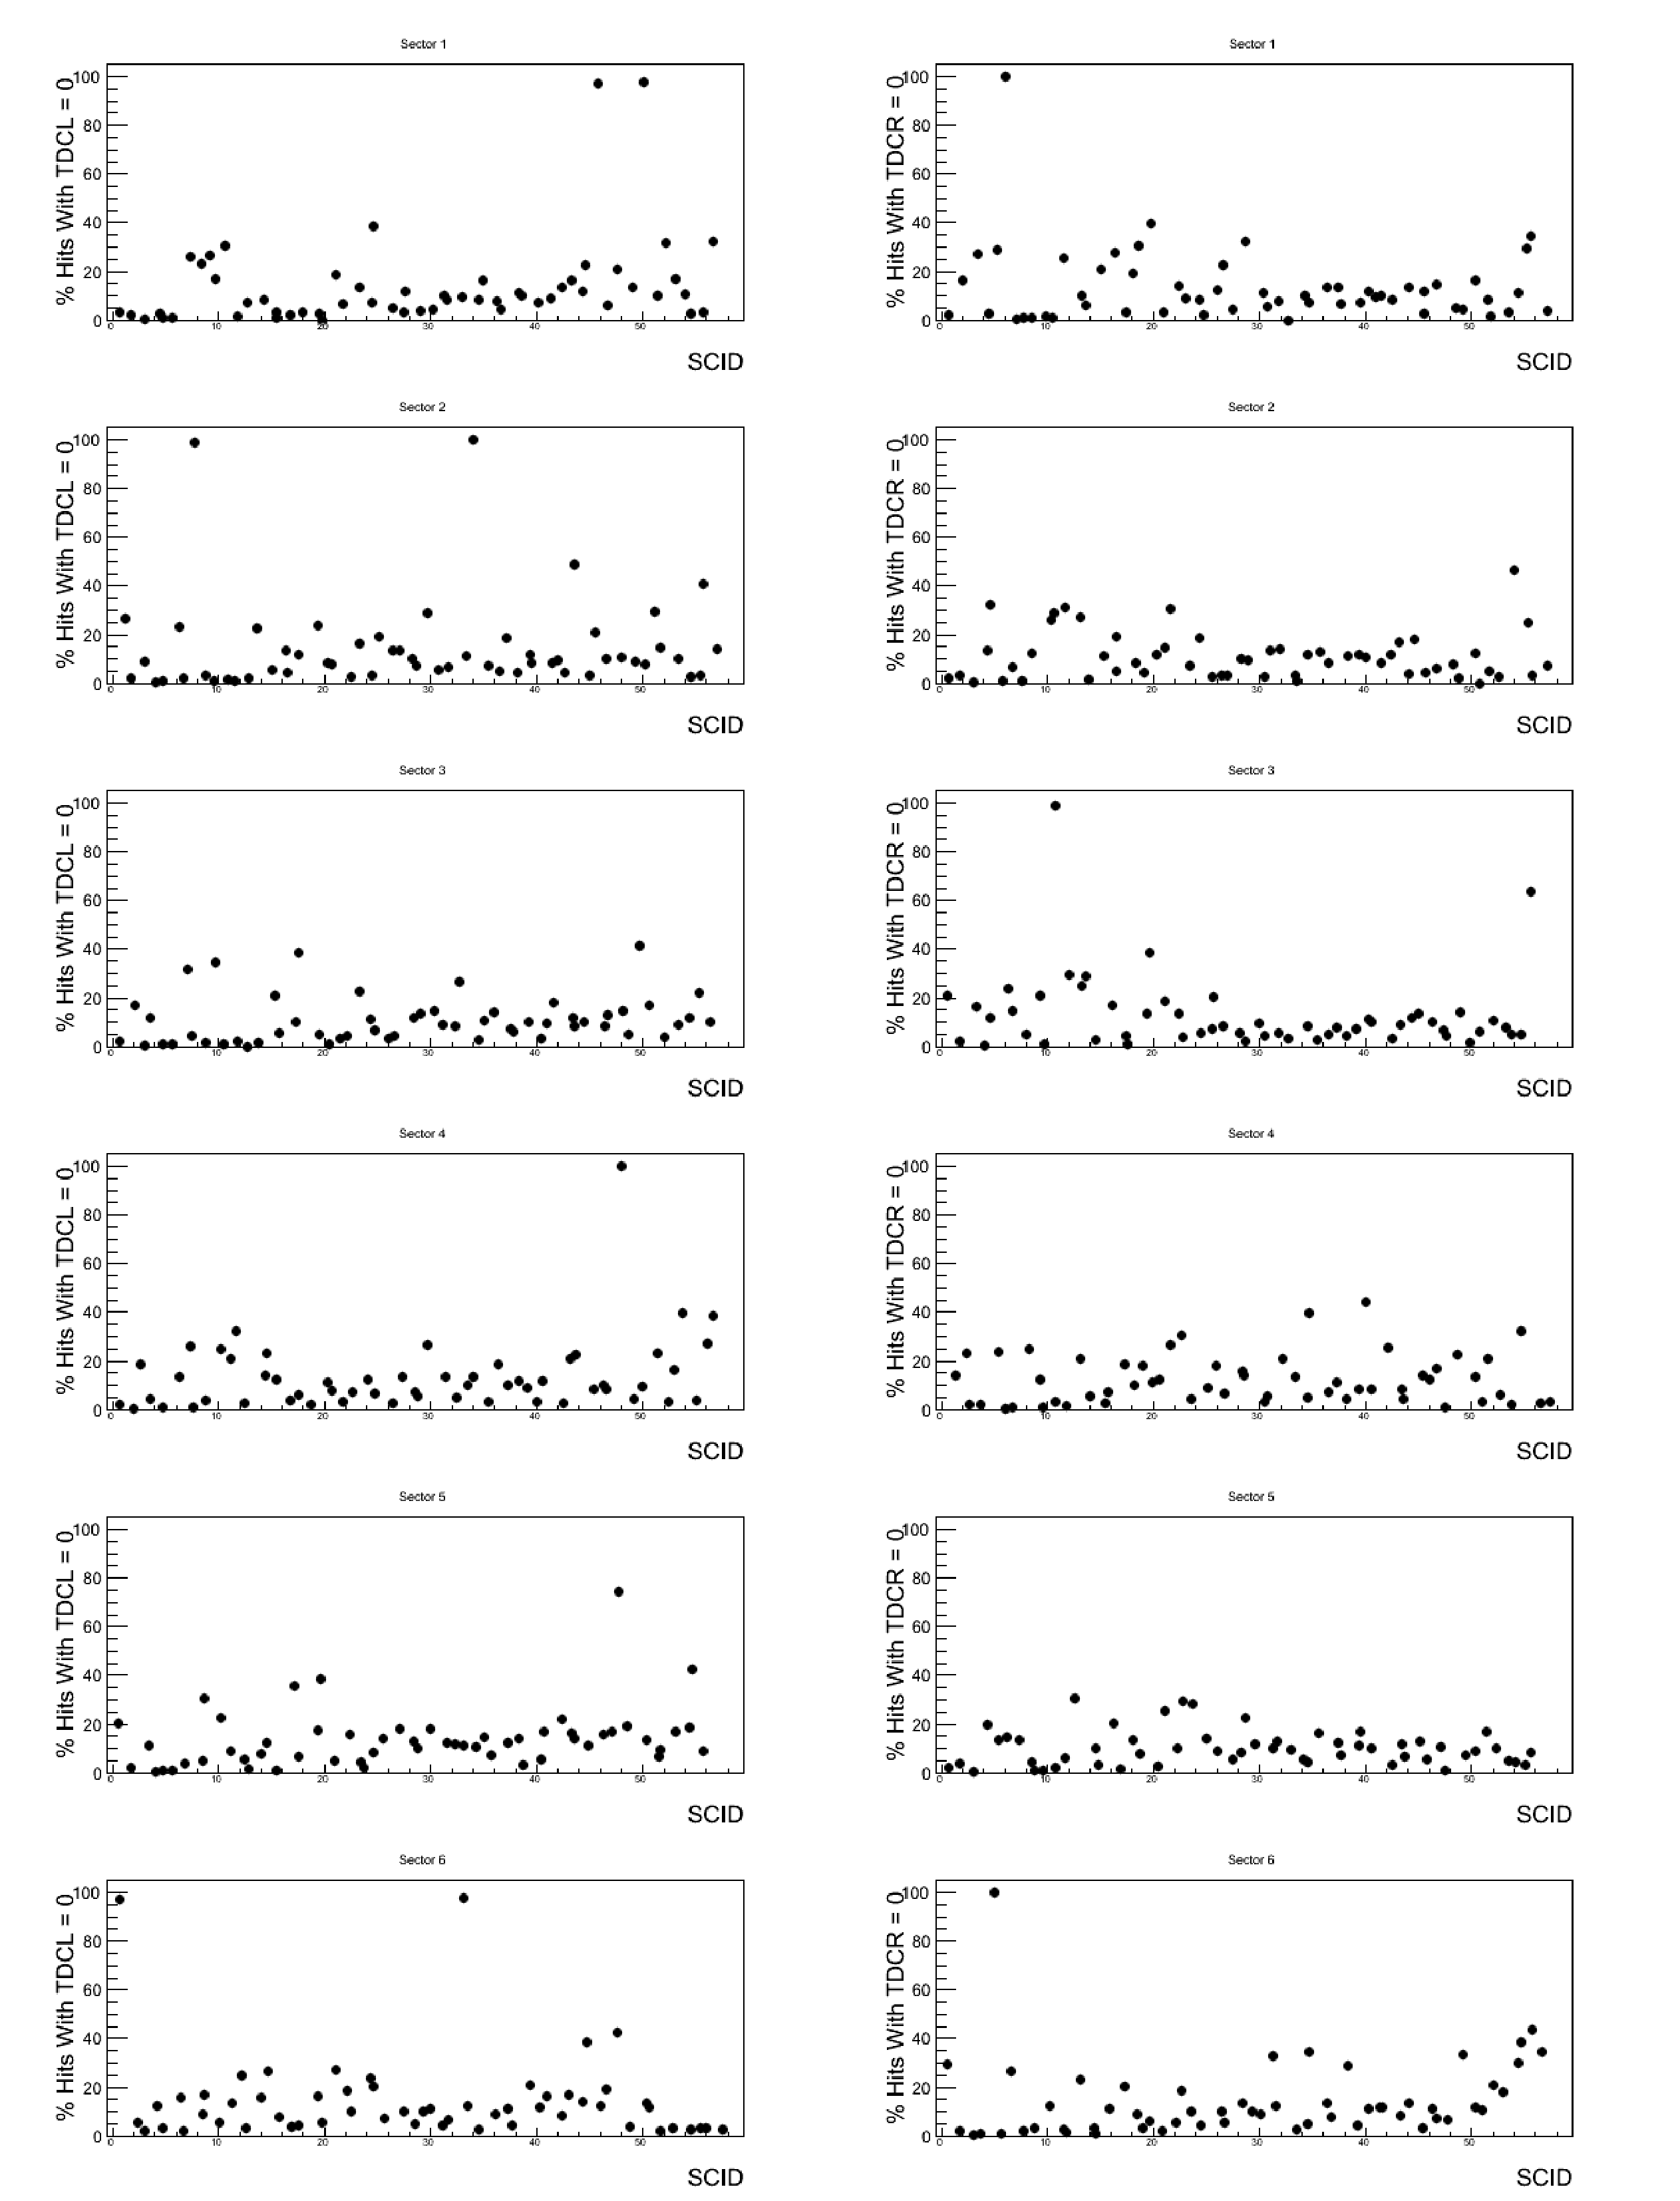
\includegraphics[width=0.8\textwidth]{figures/calib/tof/tofko/tdc.eps}
    \caption{Percentage of hits registering an TDC value of 0 for all scintillators. Left TDC (TDCL) are on the left and right TDC (TDCR) values are on the right}
    \label{plt:tdc0vSCID}
\end{figure}

\begin{figure}
    %\vspace{-16pt}
    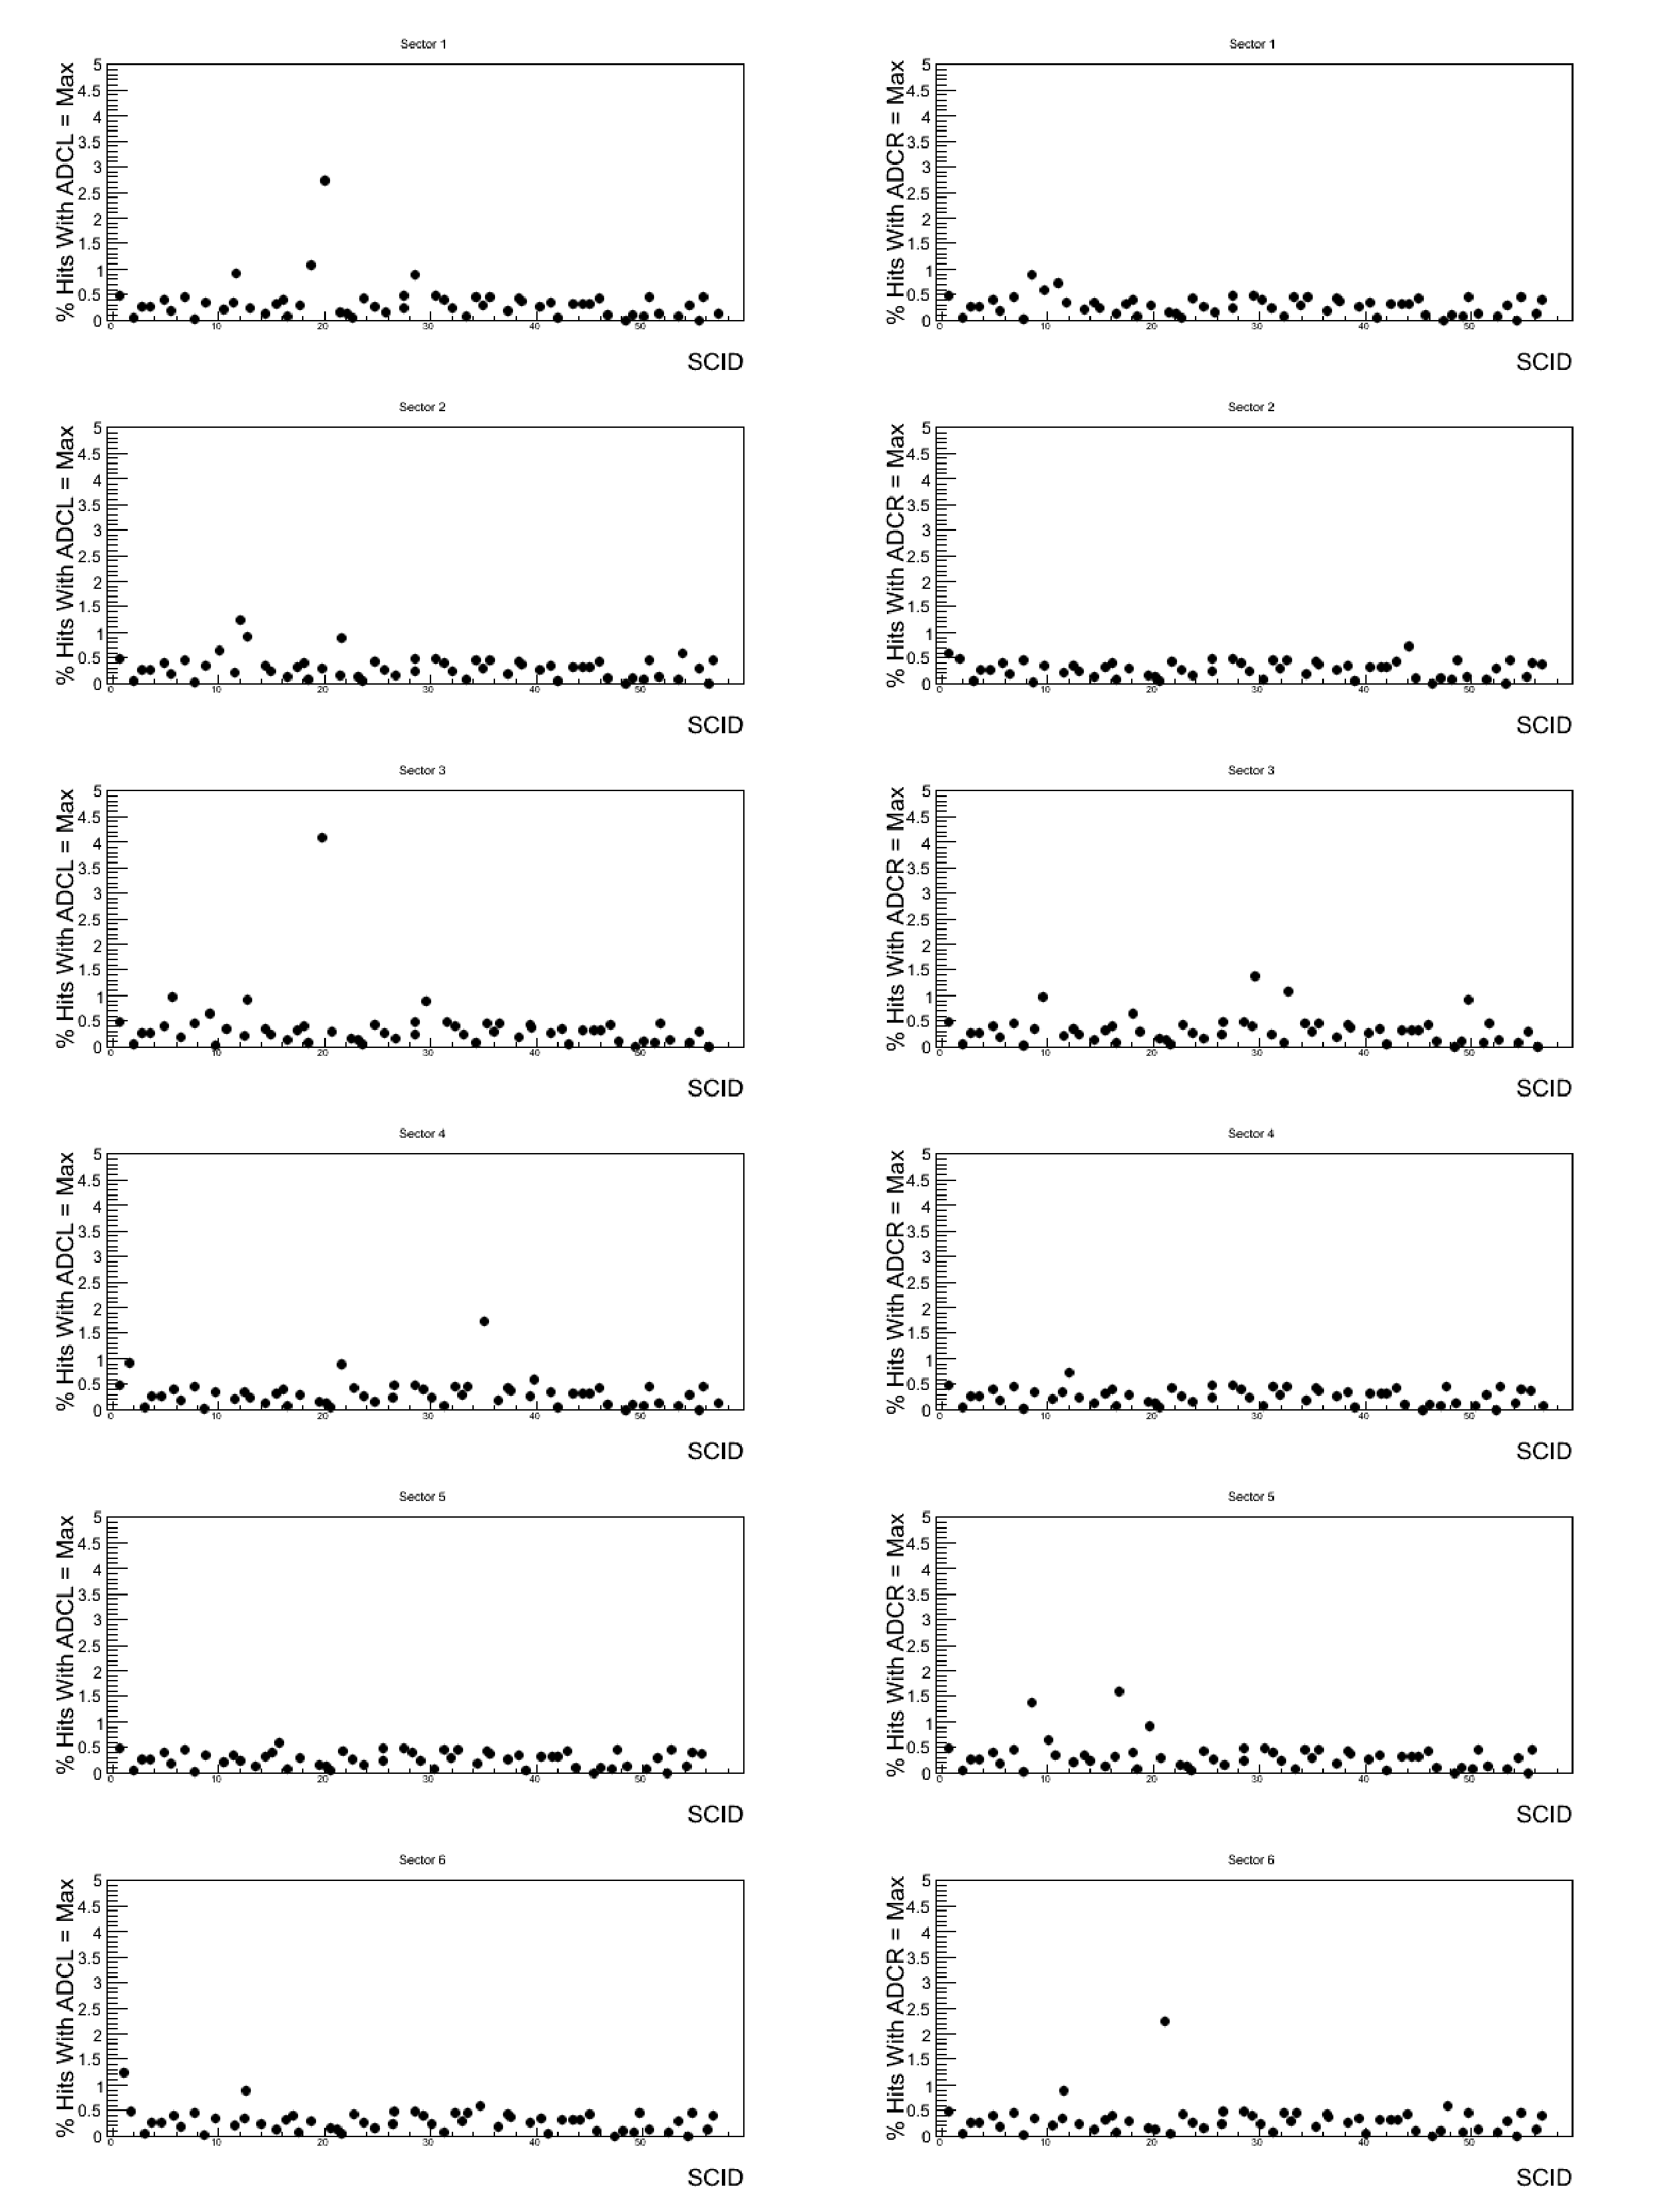
\includegraphics[width=0.8\textwidth]{figures/calib/tof/tofko/adcMax.eps}
    \caption{Percentage of hits registering a maximum ADC value for all scintillators. Left ADC (ADCL) are on the left and right ADC (ADCR) values are on the right}
    \label{plt:adcMvSCID}
\end{figure}

\begin{figure}
    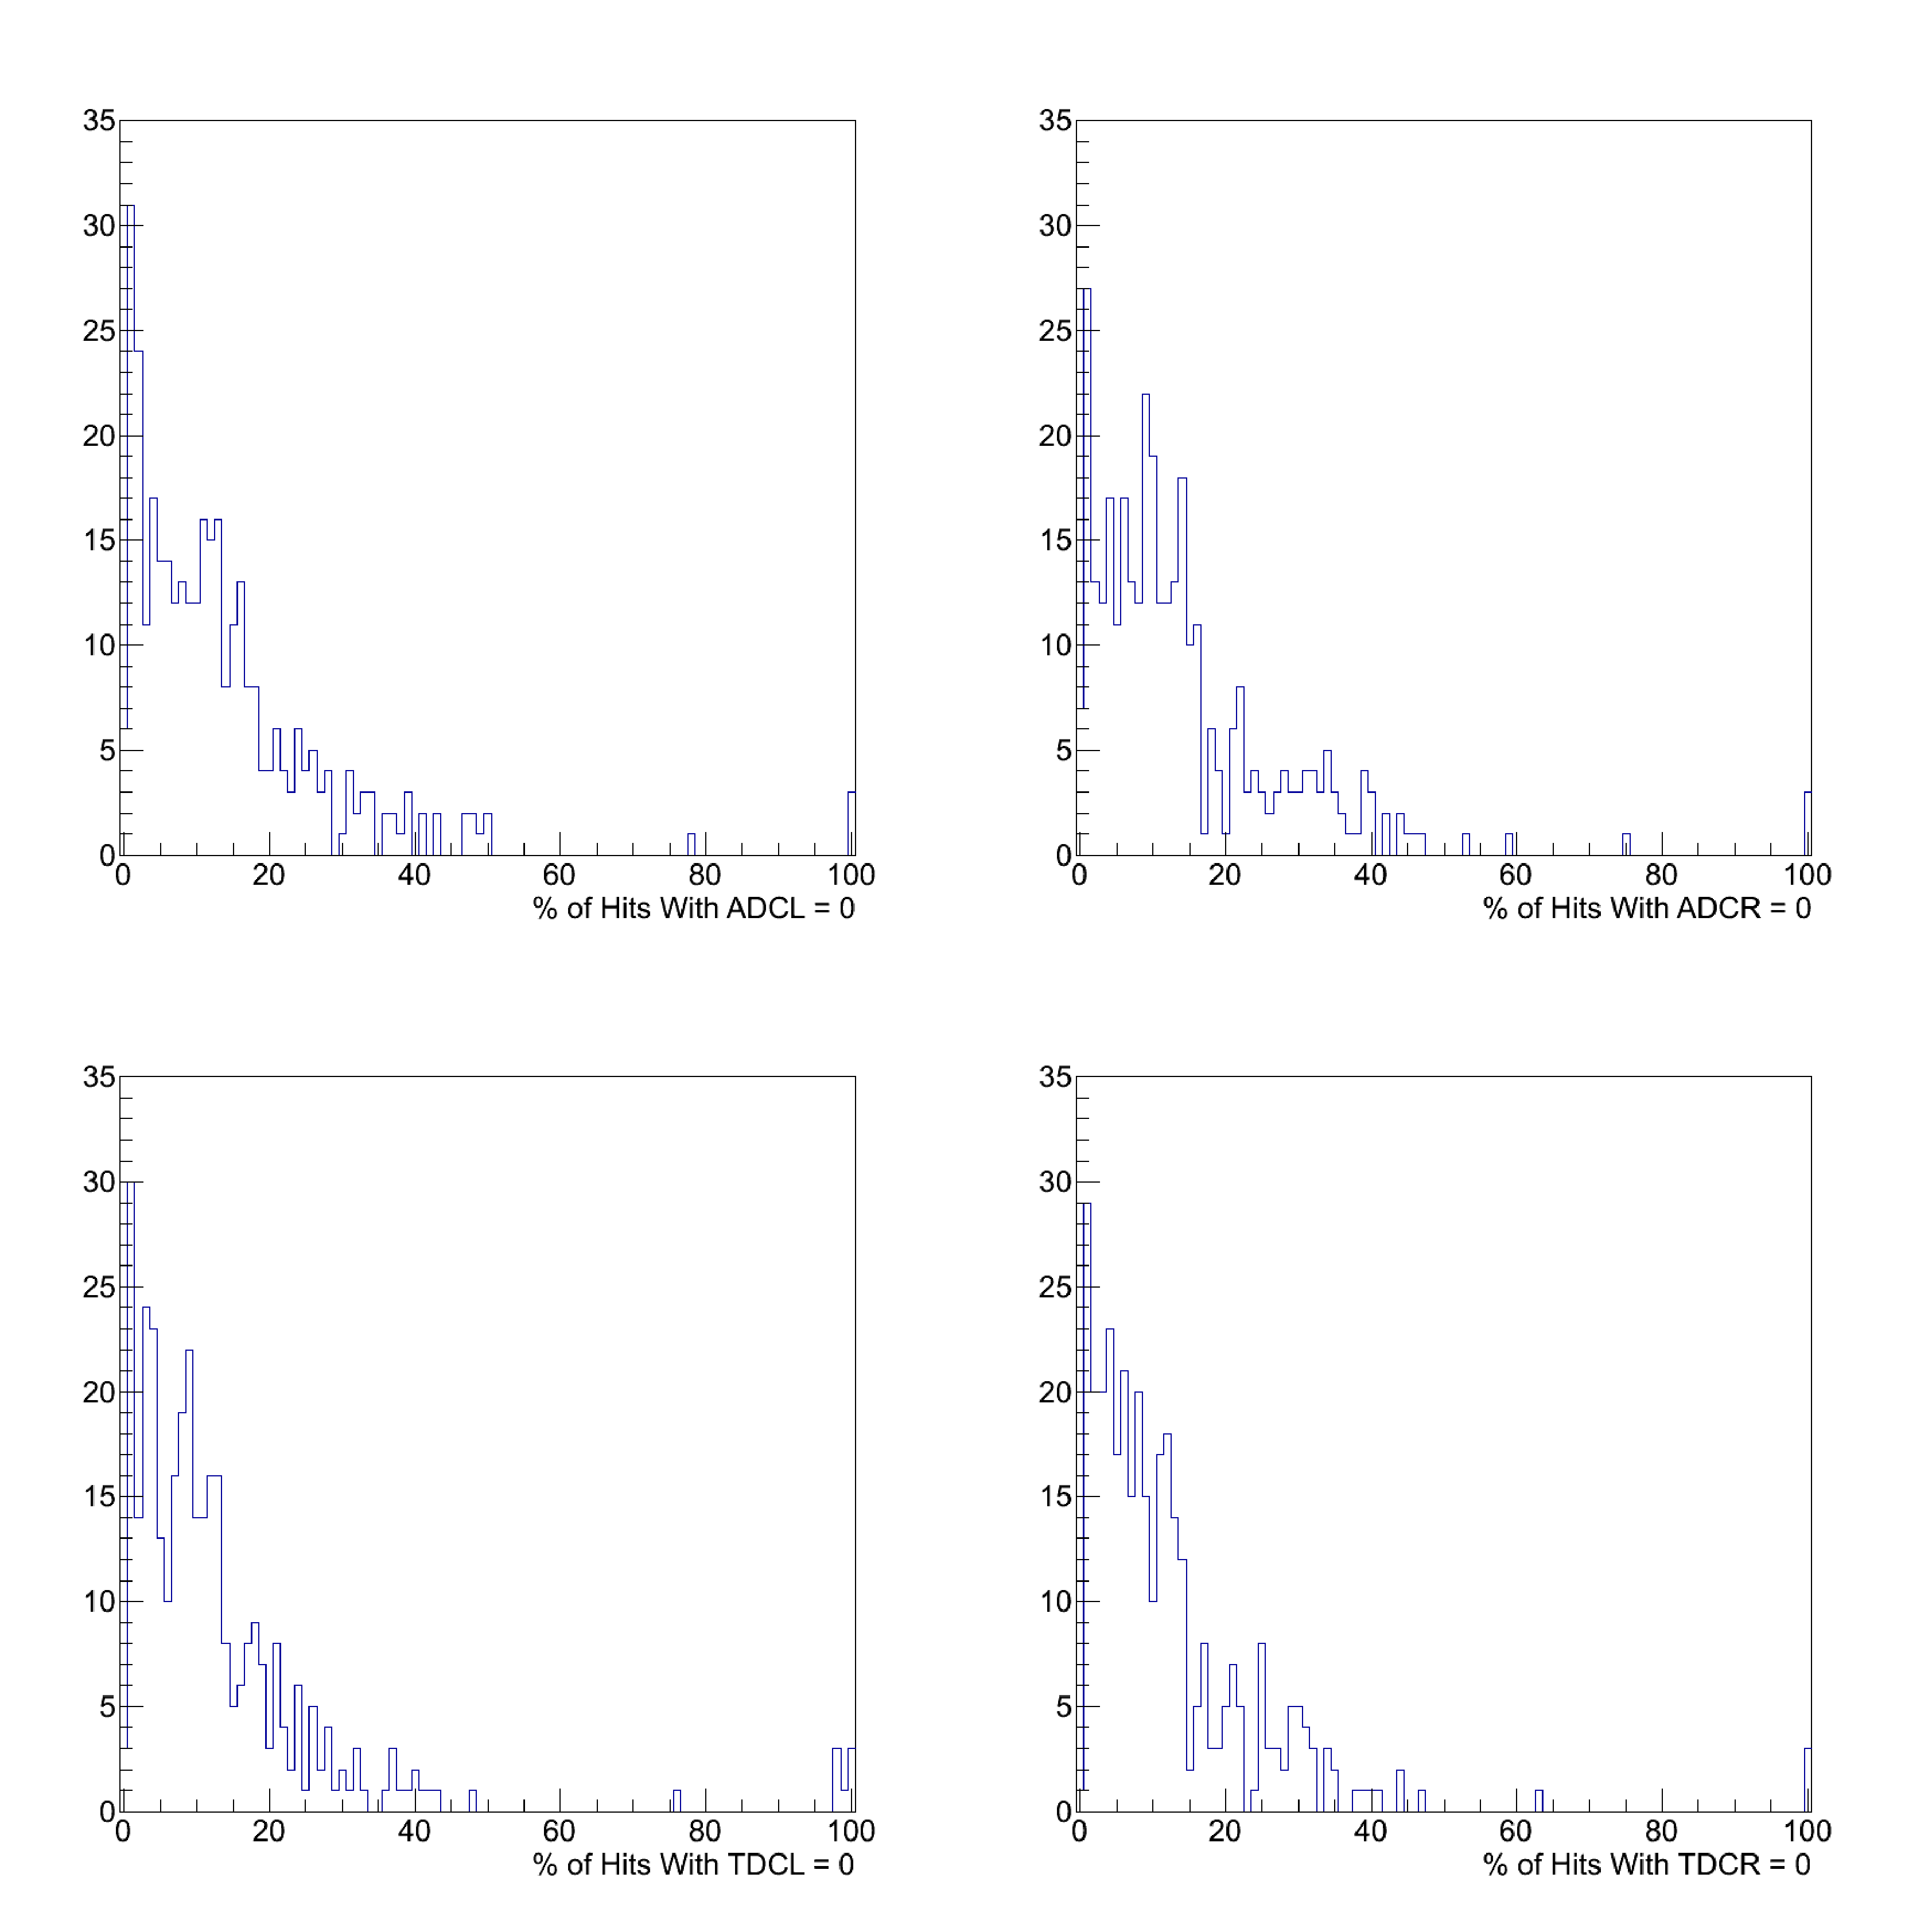
\includegraphics[width=0.8\textwidth]{figures/calib/tof/tofko/adctdc0perc.eps}
    \caption{Top: Y axis projections of \ref{plt:adc0vSCID}. Bottom: Y axis projections of \ref{plt:tdc0vSCID}}
    \label{plt:proj}
\end{figure}

\FloatBarrier
